\subsection{Motivating Datasets}\label{sec:motivating-datasets}

In principle, GLaRe can be applied to any type of complex object dataset whose observations can be stored in a vector, matrix or array. 
In this section, we introduce three motivating object datasets that can be viewed as functional data defined on two-dimensional Euclidean or spherical domains.

\subsubsection{Glaucoma Data}

Glaucoma is considered a leading factor in blindness. It is characterized by damage to the optic nerve, which can be induced by \emph{intraocular pressure (IOP)}. 
To investigate proposed hypotheses about the relationship between glaucoma and IOP, \textcite{fazio_age-related_2014} developed instrumentation to measure the mechanical strain on the scleral surface of the eye at different levels of IOP. 
The measurements were summarized for each location at different locations on the scleral surface of the eye as \emph{maximum principal strain} (MPS). MPS was computed on 34 eyes from 19 normal human donors. It was measured in the posterior globe of both eyes on a partial spherical domain with $120$ circumferential locations $\upsilon \in (0^{\circ}, 360^{\circ})$ and $120$ meridional locations $\theta \in (9^{\circ}, 24^{\circ})$.
These measurements were taken at 9 different IOP levels.
One study goal for this dataset was to test the hypothesis that scleral strain decreases with age thereby leaving the optic nerve head susceptible to damage which could be a contributing factor in the development of glaucoma \parencite{lee_bayesian_2019}.
In this work, we use a simulated copy of the real dataset that was made publicly available by \textcite{lee_bayesian_2019}\footnote{\url{https://www.tandfonline.com/doi/suppl/10.1080/01621459.2018.1476242}}.
Figure \ref{fig:combined-data-objects} (a) displays a two-dimensional polar azimuthal projection of a single observation from the Glaucoma data.

We let $X_i(t)$ denote the MPS function for a single eye at a specific IOP level so that $i = 1, \dots, N = 306$ ($34$ eyes at $9$ IOP levels).
The data lives on a domain $\mathcal{T}$ which is the portion of the sphere defined by $(\upsilon, \theta)$ for $\upsilon \in (0^{\circ}, 360^{\circ})$ and $\theta \in (9^{\circ}, 24^{\circ})$.
Therefore, each observation $X_i(t)$ is recorded a common grid of size $T = 14400$.
The recordings are indexed by the $14400$-dimensional vector $\mathbf{t} = \boldsymbol{\upsilon} \times \boldsymbol{\theta}$, where $\boldsymbol{\upsilon}$ represents $120$ equally-spaced measurements of $\upsilon$ along $(0^{\circ}, 360^{\circ})$ and $\boldsymbol{\theta}$ represents $120$ equally-spaced measurements of $\theta$ along $(9^{\circ}, 24^{\circ})$.
We denote the vector of measurements for the $i$th observation as $X_i(\mathbf{t})$, so that the full dataset can be represented by the $N \times T$ data matrix $\mathbf{X}$, containing $X_1(\mathbf{t}), \dots, X_N(\mathbf{t})$ in its rows.

\subsubsection{Proteomic Gels Data}

In neurobiology, a particularly important issue is the identification of changes responsible for the transition from non-dependent drug use to addiction which is characterized by drug intake behavior. Studies done on rats have shown that rats given a 6-12 hours/day access to cocaine or heroin have significant increase in drug intake while rats given 1 hour/day access kept the same level of intake over time.
The corresponding neurochemical changes in the extended part of the brain amygdala relate to cellular effects that affect protein expression and function which can be detected via proteomic analysis. To study this phenomenon, experiments were done on rats in which the rats were trained to get cocaine by pressing a lever: 6 rats were given 1hour/day access, 7 rats were given 6 hours /day access and 8 rats were used for control with no access to cocaine. The rats were euthanized after some time, and their brains studied \parencite{morris_pinnacle_2008}. 
Two-dimensional gel electrophoresis was used to study the proteomic content in the brain tissues. 
Between two and three gels were obtained from each rat and brain region, resulting in a dataset of 53 gel images from 21 rats.
Each gel image has $556,206$ pixel intensities observed on a $646 \times 861$ grid. 
A research goal for this dataset was to study the proteins which are differentially expressed in the brains of rats that were exposed to cocaine for a long time versus those that were not.
This can be done by finding regions in the gel images where image intensity is significantly different across groups \parencite{morris_statistical_2012}. 
Figure \ref{fig:combined-data-objects} (b) displays a single gel image observation.

We denote a single observation from the Proteomic Gels dataset as $X_i(t)$, where $i=1, \dots, N = 53$.
Here, $t$ represents a location $(t_1, t_2)$ in the two-dimensional Euclidean domain defined by the Cartesian product $\mathcal{T} = [0, 1] \times [0, 1]$.
Measurements of each observation are made at the vector of locations $\mathbf{t} = \mathbf{t}_1 \times \mathbf{t}_2$ where $\mathbf{t}_1$ and $\mathbf{t}_2$ represent vectors of $646$ and $861$ equally-spaced points along $[0, 1]$, respectively.
Then $X_i (\mathbf{t})$ denotes the $T = 556206 ( = 646 \times 861)$-dimensional vector containing the measurements of the $i$th observation at the locations in $\mathbf{t}$, and the $N \times T$ data matrix $\mathbf{X}$ contains $X_1 (\mathbf{t}), \dots, X_N (\mathbf{t})$ in its rows.


\subsubsection{MNIST Digits Data}

The MNIST (Modified National Institute of Standards and Technology) database of handwritten digits was compiled by \textcite{lecun_mnist_1998}, from a larger collection of images from the National Institute of Standards and Technology (NIST).
It comprises a training set of $60000$ images and a test set of $10000$ images, representing hand-written digits from $0$ to $9$ (i.e., $10$ distinct digits/classes).
The original black and white images from NIST were modified into $28 \times 28$ pixel greyscale images.
The MNIST dataset has been employed extensively in computer vision and deep learning applications as a test case for image reconstruction and digit identification/ classification models.
The dataset can be represented in an $N \times T$ matrix $\mathbf{X}$, where $N = 60000$ (in the case of the training set) and $T= 784$ $(= 28 \times 28)$.
We let $X_i(t)$ represent the value of the $i$th greyscale image at pixel location $t$, where $t \in \mathbf{t} = \{1, \dots, 28\} \times \{1, \dots, 28\}$.
Then the $i$th row of the data matrix $\mathbf{X}$ contains the $784$-dimensional vector $X_i(\mathbf{t})$, i.e., measurements of the $i$th observation at the vector of pixel locations in $\mathbf{t}$.
We normalise the greyscale images so that $X_i(t) \in [0, 1]$ for all $t \in \mathbf{t}$ and $i = 1, \dots, N$. 
Figure \ref{fig:combined-data-objects} (c) displays a single digit from the MNIST dataset.
The full dataset (training and test) is publicly available in the \pkg{keras} \proglang{R} package \parencite{kalinowski_keras_2024} and can be loaded using the \texttt{dataset\_mnist()} function.





\begin{figure}
    \centering
    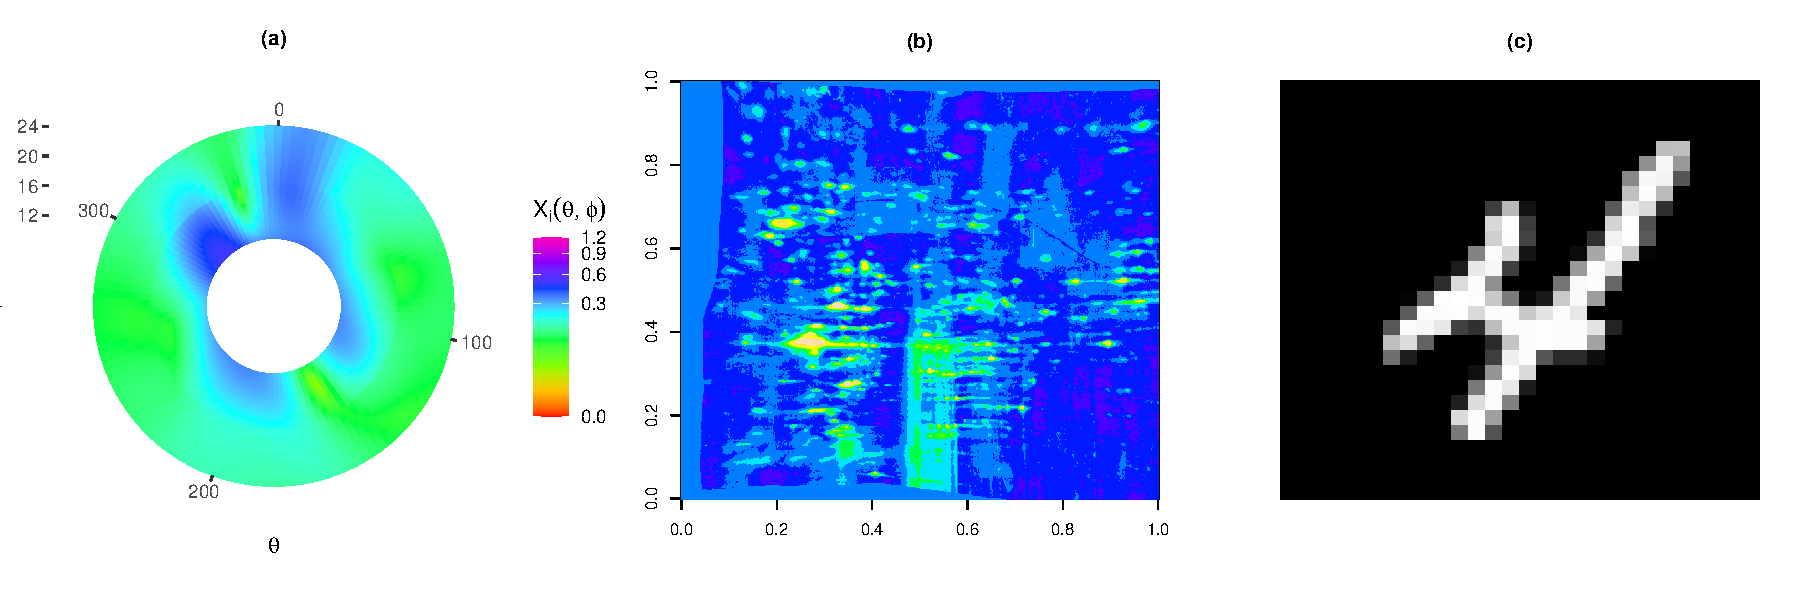
\includegraphics[width=1\textwidth]{figures/data-plot.pdf}
    \caption{
    A sample observation from each of our three motivating datasets.
    \textbf{(a)}: A sample glaucoma image, representing a polar azimuthal projection of MPS functions for a single eye at one IOP level.
    \textbf{(b)}: A sample 2D gel electrophoresis image, showing proteomic content in the brain tissue of a rat.
    \textbf{(c)}: A sample MNIST digit image, which is a $28 \times 28$ pixel greyscale image of a single handwritten digit.}
    \label{fig:combined-data-objects}
\end{figure}